\documentclass{standalone}
\usepackage{tikz}
\usetikzlibrary{patterns, positioning}


\begin{document}
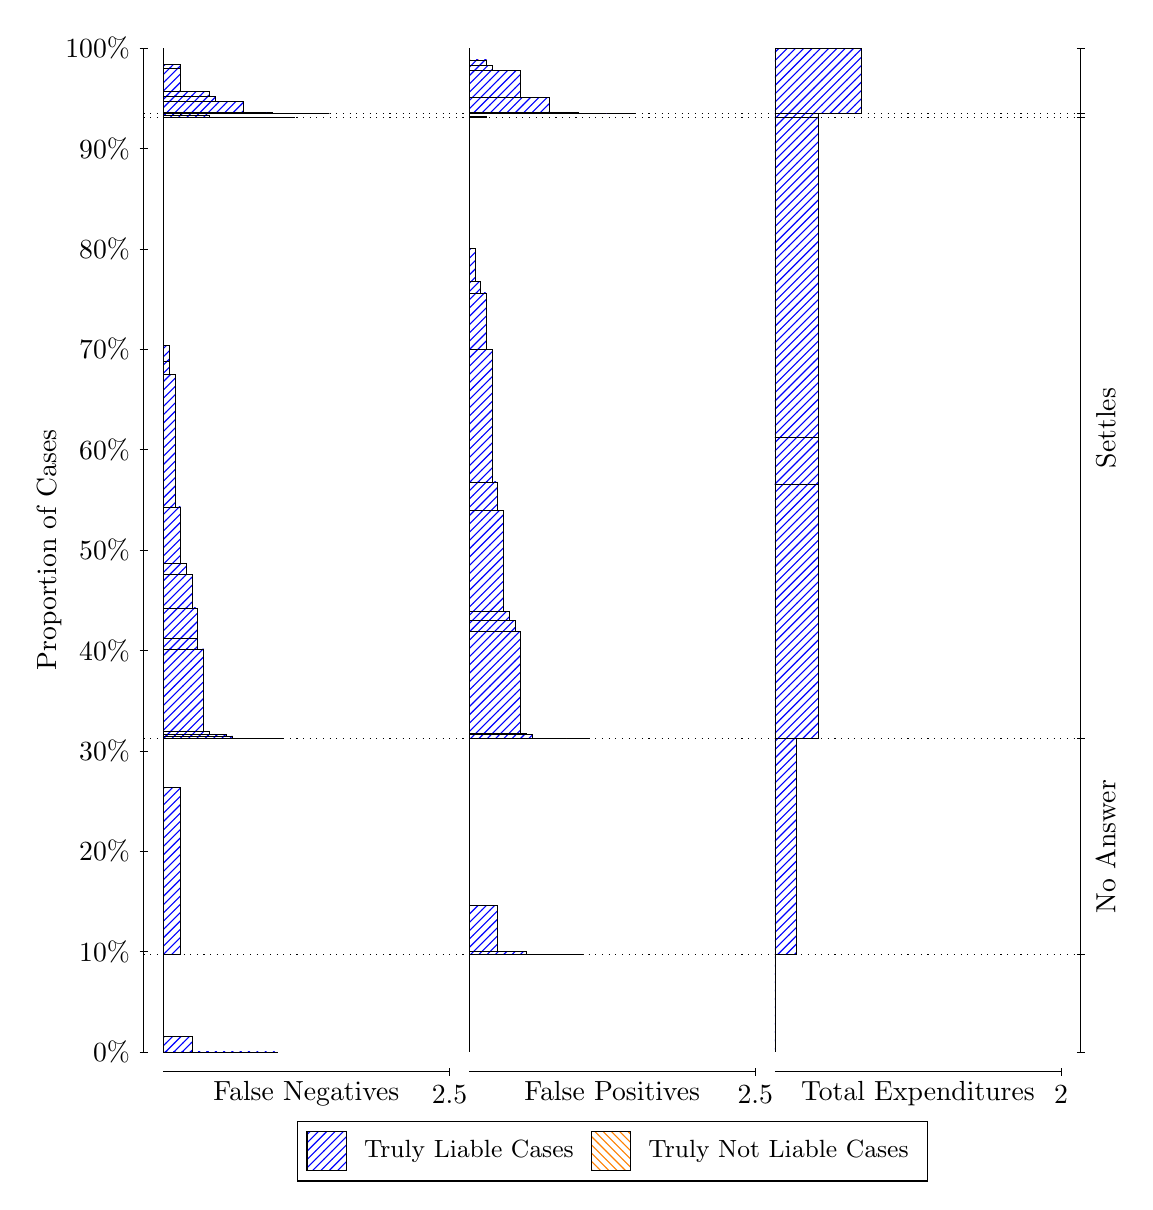
\begin{tikzpicture}
\draw[black, very thin] (1.5,1.75) -- (1.5,14.5);
\node[rotate=90, text=black, anchor=center] at (0.3, 8.125) {Proportion of Cases};
\draw[black, very thin] (1.45,1.75) -- (1.55,1.75);
\node[text=black, anchor=east] at (1.45, 1.75) {0\%};
\draw[black, very thin] (1.45,3.025) -- (1.55,3.025);
\node[text=black, anchor=east] at (1.45, 3.025) {10\%};
\draw[black, very thin] (1.45,4.3) -- (1.55,4.3);
\node[text=black, anchor=east] at (1.45, 4.3) {20\%};
\draw[black, very thin] (1.45,5.575) -- (1.55,5.575);
\node[text=black, anchor=east] at (1.45, 5.575) {30\%};
\draw[black, very thin] (1.45,6.85) -- (1.55,6.85);
\node[text=black, anchor=east] at (1.45, 6.85) {40\%};
\draw[black, very thin] (1.45,8.125) -- (1.55,8.125);
\node[text=black, anchor=east] at (1.45, 8.125) {50\%};
\draw[black, very thin] (1.45,9.4) -- (1.55,9.4);
\node[text=black, anchor=east] at (1.45, 9.4) {60\%};
\draw[black, very thin] (1.45,10.675) -- (1.55,10.675);
\node[text=black, anchor=east] at (1.45, 10.675) {70\%};
\draw[black, very thin] (1.45,11.95) -- (1.55,11.95);
\node[text=black, anchor=east] at (1.45, 11.95) {80\%};
\draw[black, very thin] (1.45,13.225) -- (1.55,13.225);
\node[text=black, anchor=east] at (1.45, 13.225) {90\%};
\draw[black, very thin] (1.45,14.5) -- (1.55,14.5);
\node[text=black, anchor=east] at (1.45, 14.5) {100\%};

\draw[black, very thin] (13.4,1.75) -- (13.4,14.5);
\draw[black, very thin] (13.35,1.75) -- (13.45,1.75);
\node[anchor=west] at (13.35, 1.75) {};
\draw[black, very thin] (13.35,2.9871) -- (13.45,2.9871);
\node[anchor=west] at (13.35, 2.9871) {};
\draw[black, very thin] (13.35,5.7325) -- (13.45,5.7325);
\node[anchor=west] at (13.35, 5.7325) {};
\draw[black, very thin] (13.35,13.615) -- (13.45,13.615);
\node[anchor=west] at (13.35, 13.615) {};
\draw[black, very thin] (13.35,13.669) -- (13.45,13.669);
\node[anchor=west] at (13.35, 13.669) {};
\draw[black, very thin] (13.35,14.5) -- (13.45,14.5);
\node[anchor=west] at (13.35, 14.5) {};

\draw[black, very thin, pattern color=blue, pattern=north east lines] (1.75,1.75) rectangle (3.2033,1.75);
\draw[black, very thin, pattern color=blue, pattern=north east lines] (1.75,1.75) rectangle (2.84,1.75);
\draw[black, very thin, pattern color=blue, pattern=north east lines] (1.75,1.75) rectangle (2.4767,1.7517);
\draw[black, very thin, pattern color=blue, pattern=north east lines] (1.75,1.7517) rectangle (2.1133,1.9526);
\draw[black, very thin, pattern color=orange, pattern=north west lines] (1.75,1.9526) rectangle (1.75,1.9526);
\draw[black, very thin, pattern color=blue, pattern=north east lines] (1.75,1.9526) rectangle (1.75,2.9871);
\draw[black, very thin, pattern color=blue, pattern=north east lines] (1.75,2.9871) rectangle (1.968,5.1055);
\draw[black, very thin, pattern color=orange, pattern=north west lines] (1.75,5.1055) rectangle (1.75,5.1055);
\draw[black, very thin, pattern color=blue, pattern=north east lines] (1.75,5.1055) rectangle (1.75,5.7325);
\draw[black, very thin, pattern color=blue, pattern=north east lines] (1.75,5.7325) rectangle (3.276,5.7325);
\draw[black, very thin, pattern color=blue, pattern=north east lines] (1.75,5.7325) rectangle (2.9853,5.7325);
\draw[black, very thin, pattern color=blue, pattern=north east lines] (1.75,5.7325) rectangle (2.9127,5.7325);
\draw[black, very thin, pattern color=blue, pattern=north east lines] (1.75,5.7325) rectangle (2.6947,5.7325);
\draw[black, very thin, pattern color=blue, pattern=north east lines] (1.75,5.7325) rectangle (2.622,5.765);
\draw[black, very thin, pattern color=blue, pattern=north east lines] (1.75,5.765) rectangle (2.5493,5.7792);
\draw[black, very thin, pattern color=blue, pattern=north east lines] (1.75,5.7792) rectangle (2.404,5.7821);
\draw[black, very thin, pattern color=blue, pattern=north east lines] (1.75,5.7821) rectangle (2.3313,5.8248);
\draw[black, very thin, pattern color=blue, pattern=north east lines] (1.75,5.8248) rectangle (2.2587,6.8683);
\draw[black, very thin, pattern color=blue, pattern=north east lines] (1.75,6.8683) rectangle (2.186,7.0067);
\draw[black, very thin, pattern color=blue, pattern=north east lines] (1.75,7.0067) rectangle (2.186,7.39);
\draw[black, very thin, pattern color=blue, pattern=north east lines] (1.75,7.39) rectangle (2.1133,7.8142);
\draw[black, very thin, pattern color=blue, pattern=north east lines] (1.75,7.8142) rectangle (2.0407,7.9577);
\draw[black, very thin, pattern color=blue, pattern=north east lines] (1.75,7.9577) rectangle (1.968,8.6712);
\draw[black, very thin, pattern color=blue, pattern=north east lines] (1.75,8.6712) rectangle (1.8953,10.358);
\draw[black, very thin, pattern color=blue, pattern=north east lines] (1.75,10.358) rectangle (1.8227,10.527);
\draw[black, very thin, pattern color=blue, pattern=north east lines] (1.75,10.527) rectangle (1.8227,10.723);
\draw[black, very thin, pattern color=orange, pattern=north west lines] (1.75,10.723) rectangle (1.75,10.723);
\draw[black, very thin, pattern color=blue, pattern=north east lines] (1.75,10.723) rectangle (1.75,13.615);
\draw[black, very thin, pattern color=blue, pattern=north east lines] (1.75,13.615) rectangle (3.4213,13.615);
\draw[black, very thin, pattern color=blue, pattern=north east lines] (1.75,13.615) rectangle (3.058,13.615);
\draw[black, very thin, pattern color=blue, pattern=north east lines] (1.75,13.615) rectangle (2.6947,13.617);
\draw[black, very thin, pattern color=blue, pattern=north east lines] (1.75,13.617) rectangle (2.3313,13.651);
\draw[black, very thin, pattern color=blue, pattern=north east lines] (1.75,13.651) rectangle (1.968,13.669);
\draw[black, very thin, pattern color=orange, pattern=north west lines] (1.75,13.669) rectangle (1.75,13.669);
\draw[black, very thin, pattern color=blue, pattern=north east lines] (1.75,13.669) rectangle (3.8573,13.669);
\draw[black, very thin, pattern color=blue, pattern=north east lines] (1.75,13.669) rectangle (3.494,13.669);
\draw[black, very thin, pattern color=blue, pattern=north east lines] (1.75,13.669) rectangle (3.1307,13.685);
\draw[black, very thin, pattern color=blue, pattern=north east lines] (1.75,13.685) rectangle (3.058,13.685);
\draw[black, very thin, pattern color=blue, pattern=north east lines] (1.75,13.685) rectangle (2.7673,13.819);
\draw[black, very thin, pattern color=blue, pattern=north east lines] (1.75,13.819) rectangle (2.6947,13.819);
\draw[black, very thin, pattern color=blue, pattern=north east lines] (1.75,13.819) rectangle (2.404,13.892);
\draw[black, very thin, pattern color=blue, pattern=north east lines] (1.75,13.892) rectangle (2.3313,13.952);
\draw[black, very thin, pattern color=blue, pattern=north east lines] (1.75,13.952) rectangle (2.0407,13.953);
\draw[black, very thin, pattern color=blue, pattern=north east lines] (1.75,13.953) rectangle (1.968,14.247);
\draw[black, very thin, pattern color=blue, pattern=north east lines] (1.75,14.247) rectangle (1.968,14.296);
\draw[black, very thin, pattern color=orange, pattern=north west lines] (1.75,14.296) rectangle (1.75,14.296);
\draw[black, very thin, pattern color=blue, pattern=north east lines] (1.75,14.296) rectangle (1.75,14.5);
\draw[black, very thin, pattern color=orange, pattern=north west lines] (5.6333,1.75) rectangle (5.6333,1.75);
\draw[black, very thin, pattern color=blue, pattern=north east lines] (5.6333,1.75) rectangle (5.6333,2.9871);
\draw[black, very thin, pattern color=orange, pattern=north west lines] (5.6333,2.9871) rectangle (7.0867,2.9871);
\draw[black, very thin, pattern color=blue, pattern=north east lines] (5.6333,2.9871) rectangle (7.0867,2.9871);
\draw[black, very thin, pattern color=blue, pattern=north east lines] (5.6333,2.9871) rectangle (6.7233,2.9874);
\draw[black, very thin, pattern color=blue, pattern=north east lines] (5.6333,2.9874) rectangle (6.36,3.0323);
\draw[black, very thin, pattern color=blue, pattern=north east lines] (5.6333,3.0323) rectangle (5.9967,3.6141);
\draw[black, very thin, pattern color=blue, pattern=north east lines] (5.6333,3.6141) rectangle (5.6333,5.7325);
\draw[black, very thin, pattern color=orange, pattern=north west lines] (5.6333,5.7325) rectangle (7.1593,5.7325);
\draw[black, very thin, pattern color=blue, pattern=north east lines] (5.6333,5.7325) rectangle (7.1593,5.7325);
\draw[black, very thin, pattern color=orange, pattern=north west lines] (5.6333,5.7325) rectangle (6.8687,5.7325);
\draw[black, very thin, pattern color=blue, pattern=north east lines] (5.6333,5.7325) rectangle (6.8687,5.7325);
\draw[black, very thin, pattern color=blue, pattern=north east lines] (5.6333,5.7325) rectangle (6.796,5.7325);
\draw[black, very thin, pattern color=orange, pattern=north west lines] (5.6333,5.7325) rectangle (6.7233,5.7325);
\draw[black, very thin, pattern color=blue, pattern=north east lines] (5.6333,5.7325) rectangle (6.7233,5.7325);
\draw[black, very thin, pattern color=orange, pattern=north west lines] (5.6333,5.7325) rectangle (6.578,5.7325);
\draw[black, very thin, pattern color=blue, pattern=north east lines] (5.6333,5.7325) rectangle (6.578,5.7347);
\draw[black, very thin, pattern color=blue, pattern=north east lines] (5.6333,5.7347) rectangle (6.5053,5.735);
\draw[black, very thin, pattern color=blue, pattern=north east lines] (5.6333,5.735) rectangle (6.4327,5.7902);
\draw[black, very thin, pattern color=blue, pattern=north east lines] (5.6333,5.7902) rectangle (6.36,5.7919);
\draw[black, very thin, pattern color=orange, pattern=north west lines] (5.6333,5.7919) rectangle (6.2873,5.7919);
\draw[black, very thin, pattern color=blue, pattern=north east lines] (5.6333,5.7919) rectangle (6.2873,7.0889);
\draw[black, very thin, pattern color=blue, pattern=north east lines] (5.6333,7.0889) rectangle (6.2147,7.2316);
\draw[black, very thin, pattern color=blue, pattern=north east lines] (5.6333,7.2316) rectangle (6.142,7.3441);
\draw[black, very thin, pattern color=blue, pattern=north east lines] (5.6333,7.3441) rectangle (6.0693,8.6243);
\draw[black, very thin, pattern color=orange, pattern=north west lines] (5.6333,8.6243) rectangle (5.9967,8.6243);
\draw[black, very thin, pattern color=blue, pattern=north east lines] (5.6333,8.6243) rectangle (5.9967,8.9898);
\draw[black, very thin, pattern color=blue, pattern=north east lines] (5.6333,8.9898) rectangle (5.924,10.677);
\draw[black, very thin, pattern color=blue, pattern=north east lines] (5.6333,10.677) rectangle (5.8513,11.39);
\draw[black, very thin, pattern color=blue, pattern=north east lines] (5.6333,11.39) rectangle (5.7787,11.534);
\draw[black, very thin, pattern color=blue, pattern=north east lines] (5.6333,11.534) rectangle (5.706,11.958);
\draw[black, very thin, pattern color=blue, pattern=north east lines] (5.6333,11.958) rectangle (5.6333,13.615);
\draw[black, very thin, pattern color=orange, pattern=north west lines] (5.6333,13.615) rectangle (5.8513,13.615);
\draw[black, very thin, pattern color=blue, pattern=north east lines] (5.6333,13.615) rectangle (5.8513,13.633);
\draw[black, very thin, pattern color=blue, pattern=north east lines] (5.6333,13.633) rectangle (5.6333,13.669);
\draw[black, very thin, pattern color=orange, pattern=north west lines] (5.6333,13.669) rectangle (7.7407,13.669);
\draw[black, very thin, pattern color=blue, pattern=north east lines] (5.6333,13.669) rectangle (7.7407,13.669);
\draw[black, very thin, pattern color=orange, pattern=north west lines] (5.6333,13.669) rectangle (7.3773,13.669);
\draw[black, very thin, pattern color=blue, pattern=north east lines] (5.6333,13.669) rectangle (7.3773,13.669);
\draw[black, very thin, pattern color=orange, pattern=north west lines] (5.6333,13.669) rectangle (7.014,13.669);
\draw[black, very thin, pattern color=blue, pattern=north east lines] (5.6333,13.669) rectangle (7.014,13.68);
\draw[black, very thin, pattern color=orange, pattern=north west lines] (5.6333,13.68) rectangle (6.6507,13.68);
\draw[black, very thin, pattern color=blue, pattern=north east lines] (5.6333,13.68) rectangle (6.6507,13.872);
\draw[black, very thin, pattern color=orange, pattern=north west lines] (5.6333,13.872) rectangle (6.578,13.872);
\draw[black, very thin, pattern color=blue, pattern=north east lines] (5.6333,13.872) rectangle (6.578,13.872);
\draw[black, very thin, pattern color=blue, pattern=north east lines] (5.6333,13.872) rectangle (6.2873,14.216);
\draw[black, very thin, pattern color=orange, pattern=north west lines] (5.6333,14.216) rectangle (6.2147,14.216);
\draw[black, very thin, pattern color=blue, pattern=north east lines] (5.6333,14.216) rectangle (6.2147,14.216);
\draw[black, very thin, pattern color=blue, pattern=north east lines] (5.6333,14.216) rectangle (5.924,14.276);
\draw[black, very thin, pattern color=blue, pattern=north east lines] (5.6333,14.276) rectangle (5.8513,14.349);
\draw[black, very thin, pattern color=orange, pattern=north west lines] (5.6333,14.349) rectangle (5.8513,14.349);
\draw[black, very thin, pattern color=blue, pattern=north east lines] (5.6333,14.349) rectangle (5.8513,14.35);
\draw[black, very thin, pattern color=blue, pattern=north east lines] (5.6333,14.35) rectangle (5.6333,14.5);
\draw[black, very thin, pattern color=orange, pattern=north west lines] (9.5167,1.75) rectangle (9.5167,1.75);
\draw[black, very thin, pattern color=blue, pattern=north east lines] (9.5167,1.75) rectangle (9.5167,2.9871);
\draw[black, very thin, pattern color=orange, pattern=north west lines] (9.5167,2.9871) rectangle (9.7892,2.9871);
\draw[black, very thin, pattern color=blue, pattern=north east lines] (9.5167,2.9871) rectangle (9.7892,5.7325);
\draw[black, very thin, pattern color=orange, pattern=north west lines] (9.5167,5.7325) rectangle (10.062,5.7325);
\draw[black, very thin, pattern color=blue, pattern=north east lines] (9.5167,5.7325) rectangle (10.062,8.9618);
\draw[black, very thin, pattern color=orange, pattern=north west lines] (9.5167,8.9618) rectangle (10.062,8.9618);
\draw[black, very thin, pattern color=blue, pattern=north east lines] (9.5167,8.9618) rectangle (10.062,9.5556);
\draw[black, very thin, pattern color=orange, pattern=north west lines] (9.5167,9.5556) rectangle (10.062,9.5556);
\draw[black, very thin, pattern color=blue, pattern=north east lines] (9.5167,9.5556) rectangle (10.062,13.615);
\draw[black, very thin, pattern color=orange, pattern=north west lines] (9.5167,13.615) rectangle (10.062,13.615);
\draw[black, very thin, pattern color=blue, pattern=north east lines] (9.5167,13.615) rectangle (10.062,13.669);
\draw[black, very thin, pattern color=orange, pattern=north west lines] (9.5167,13.669) rectangle (10.607,13.669);
\draw[black, very thin, pattern color=blue, pattern=north east lines] (9.5167,13.669) rectangle (10.607,14.5);
\draw[black, dotted] (1.5,2.9871) -- (13.4,2.9871);
\draw[black, dotted] (1.5,5.7325) -- (13.4,5.7325);
\draw[black, dotted] (1.5,13.615) -- (13.4,13.615);
\draw[black, dotted] (1.5,13.669) -- (13.4,13.669);
\draw[black, very thin] (1.75,1.5) -- (5.3833,1.5);
\node[text=black, anchor=north] at (3.5667, 1.5) {False Negatives};
\draw[black, very thin] (5.3833,1.45) -- (5.3833,1.55);
\node[text=black, anchor=north] at (5.3833, 1.45) {2.5};

\draw[black, very thin] (5.6333,1.5) -- (9.2667,1.5);
\node[text=black, anchor=north] at (7.45, 1.5) {False Positives};
\draw[black, very thin] (9.2667,1.45) -- (9.2667,1.55);
\node[text=black, anchor=north] at (9.2667, 1.45) {2.5};

\draw[black, very thin] (9.5167,1.5) -- (13.15,1.5);
\node[text=black, anchor=north] at (11.333, 1.5) {Total Expenditures};
\draw[black, very thin] (13.15,1.45) -- (13.15,1.55);
\node[text=black, anchor=north] at (13.15, 1.45) {2};


\node[text=black, centered, rotate=90] at (13.72, 4.3598) {No Answer};
\node[text=black, centered, rotate=90] at (13.72, 9.6739) {Settles};



\draw (7.449999999999999,1.5) node[draw=none] (baseCoordinate) {};
\begin{scope}[align=center]
        \matrix[scale=0.5, draw=black, below=0.5cm of baseCoordinate, nodes={draw}, column sep=0.1cm]{
            \node[rectangle, draw, minimum width=0.5cm, minimum height=0.5cm, pattern color=blue, pattern=north east lines] {}; &
            \node[draw=none, font=\small, text=black] (B) {Truly Liable Cases}; &
            \node[rectangle, draw, minimum width=0.5cm, minimum height=0.5cm, pattern color=orange, pattern=north west lines] {}; &
            \node[draw=none, font=\small, text=black] (B) {Truly Not Liable Cases}; \\
            };
\end{scope}

\end{tikzpicture}
\end{document}